\let\RaggedRight\raggedright
\let\raggedright\relax
\documentclass[utf8,9pt,mathserif,usepdftitle=false]{beamer}
\usepackage[russian]{babel}

\newcommand{\dd}{\mathrm{d}}
\renewcommand{\Re}{\operatorname{Re}}
\renewcommand{\Im}{\operatorname{Im}}
\renewcommand{\exp}{\operatorname{e}}
\renewcommand{\imath}{\mathrm{i}}

% \input{present.daf}

% \setbeameroption{show notes on second screen}
\setbeameroption{hide notes}
\mode<presentation>
{
  \usetheme{default}
  %\usecolortheme{default} % dove, beaver
  \usecolortheme{whale}
  %\usefonttheme{serif}
}

\hypersetup{%
  pdfinfo={%
    Title={Lyapunov conference, IDSTU},%
    Subject={Spin degrees of freedom for fermion systems},%
    Author={Даниил Кучеров},%
    Keywords={fermion polarization;fermion spinor projection}%
  }
}

\title{Зависимость вероятности выживания электронного нейтрино от углов
  смешивания}%
\author{\underline{Кучеров Д.А.}\\[7em]\raggedleft\footnotesize Научный руководитель:
  Ломов В.П.\\%
}%
\date[ИГУ, 2025]{\vfill%\\[4ex]%
  \small{}Иркутск, 2025}

\begin{document}
\begin{frame}
  \titlepage
\end{frame}

\begin{frame}
	\frametitle{Задачи работы}
  В работе поставленно несколько задач:
  \begin{itemize}
  \item<2-> Изучить теорию нейтринных осцилляций в среде, разобрать используемую модель.
  \item<3-> Провести вычисления с помощью метода разложения Магнуса, варьируя значения углов смешивания.
  \item<4-> Проанализировать полученные решения.
  \item<5-> Сделать вывод об характере зависимости вероятности выживания электронного нейтрино от значения углов смешивания. 
  \end{itemize}
\end{frame}

\begin{frame}
	\frametitle{Теоритическая часть}%
	Нейтрино можно классифицировать по двум критериям: по массе и по их связи с
  заряженными лептонами (по флейворам).

  \onslide<2->%
	В физике элементарных частиц, термин «флейвор» используется для описания
  различных типов элементарных частиц. Этот термин часто применяется в отношении
  кварков и лептонов, включая нейтрино.

  \onslide<3->%	
	Нейтрино существуют в трех флейворах: электронные, мюонные и
  тау-нейтрино. Каждый флейвор ассоциируется с соответствующим лептоном
  (электроном, мюоном и тау-лептоном). Эти флейворы нейтрино уникальны тем, что
  они могут меняться один в другой в процессе нейтринных осцилляций.

  \onslide<4->%
  Переход нейтрино из одного флейвора в другой описывается уравнением:
	\begin{equation}
		|\nu_{\alpha}\rangle=\sum_{i}U_{\alpha i}^{*}|\nu_{i}\rangle
	\end{equation}
\end{frame}

\begin{frame}
	\frametitle{Уравнение нейтринных осцилляций}%
	Когда активные флэйворные нейтрино распространяются в веществе, на их
  эволюционное уравнение влияют эффективные потенциалы из-за когерентного
  взаимодействия со средой посредством реакций нейтрального и заряженного
  токов. Таким образом, влияние среды можно описать в терминах потенциалов, в
  которых распространяются нейтрино, зависящим от состава среды, электрической
  нейтральности, намагниченности (ориентации спинов), скоростей частиц
  среды. Учитывая данные обстоятельства, было выведено уравнение:
	\begin{equation}\label{eq:2}
		\imath\frac{\dd\psi}{\dd\xi}=[H_{0}+\nu(\xi)W]\psi
	\end{equation}
	Оно имеет несколько особенностей: уравнение матричное, состоящее из трёх
  компонент, \(H(\xi)=[H_{0}+\nu(\xi)W]\) это унитарная матрица гамильтониана
  эволюции.  Данное уравнение на сегодняшний день не имеет аналитического
  решения. А численное интегрирование достаточно трудоёмкий процесс.
\end{frame}

\begin{frame}
	\frametitle{Метод разложения Магнуса}%
	Одним из способов интегрирования уравнения \eqref{eq:2} является метод
  разложения Магнуса. Этот метод относится к так называемым геометрическим
  интеграторам, которые заточены под решения таких дифференциальных уравнений
  как \eqref{eq:2}. Отличительной особенностью разложения Магнуса является то,
  что приближенное решение, предоставляемое процедурой, разделяет с точным
  решением соответствующие геометрические свойства. В нашем случае этим
  свойством является унитарность оператора эволюции времени.
\end{frame}

\begin{frame}
	\frametitle{Генерирование и обработка данных}%
  Для автоматизации процесса генерации и обработки данных были написаны сценарии
  в bash-оболочке. Уравнение нейтринных осцилляций было численно решено с
  помощью программы m4-tol.
	
	Для оценки точности мы воспользуемся одним замечательным свойством уравнения
  \eqref{eq:2}, а именно сохранение нормировки, то есть решение имеет смысл
  вероятности, а это значит, что будет справедливо выражение
  \(\sum_{i}|\psi_{i}|^{2}-1=0\). Далее интегрируем уравнение \eqref{eq:2},
  используя метод Рунге-Кутты реализованный в wolfram mathematica (используемая
  версия 13.2.1.0), в диапазоне от 0,1 до 1. Затем, записываем в файл решение в
  диапазоне от 0,101 до 1 с шагом \(10^{-3}\). С помощью python строим график
  функции \(F(\xi)=\sum_{i}|\psi_{i}(\xi)|^{2}-1\)
	
	Проводим подобную процедуру и для метода разложения Магнуса.
\end{frame}

\begin{frame}
  \begin{figure}[h]
		\centering	
		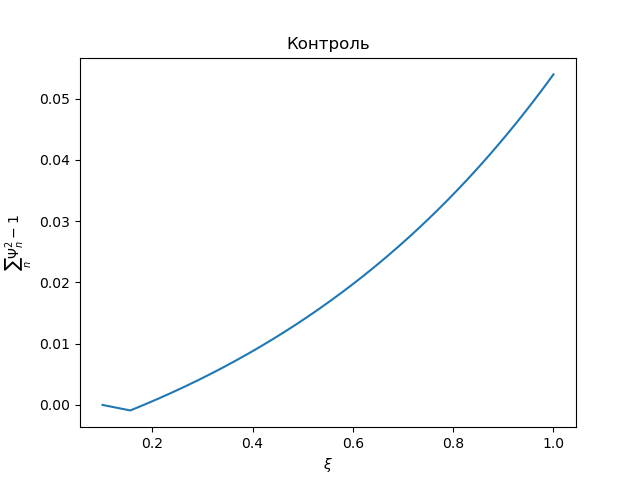
\includegraphics[width=0.8\linewidth]{контроль_м}
		\caption{График контроля нормировки для решения полученного с помощью wolfram mathematica}
	\end{figure}
\end{frame}

\begin{frame}
	\begin{figure}[h]
		\centering	
		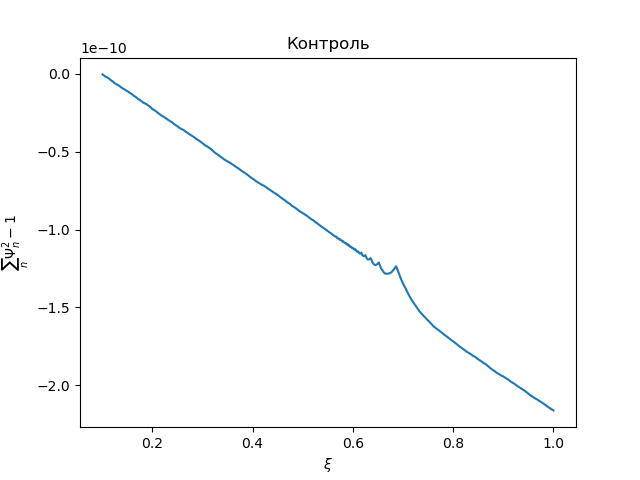
\includegraphics[width=0.8\linewidth]{контроль_магнус}
		\caption{График контроля нормировки для решения полученного с помощью метода разложения Магнуса}
	\end{figure}
\end{frame}

\begin{frame}
	\begin{figure}[h]

	\frametitle{Вывод}
	Из полученных графиков, можно сделать вывод, что метод разложения Магнуса является достаточно эффективным методом интегрирования уравнения \eqref{eq:2}, в сравнении с методом Рунге-Кутты.
	
	\end{figure}
\end{frame}

\begin{frame}
  \frametitle{КОНЕЦ}
  \LARGE\centering\bfseries
  СПАСИБО ЗА ВНИМАНИЕ!
\end{frame}

\begin{frame}
  \frametitle{Дополнительный материал}
\end{frame}

\end{document}

%%% Local Variables:
%%% mode: latex
%%% fill-column: 80
%%% TeX-master: t
%%% TeX-PDF-mode: t
%%% End:
%%% vim: syn=tex ft=tex tw=80 ts=2 sw=2 et:
